% Author: K4YT3X
% Date Created: Sep 23, 2018

% Template downloaded from: http://www.LaTeXTemplates.com
% Original author: WikiBooks
% License:
% CC BY-NC-SA 3.0 (http://creativecommons.org/licenses/by-nc-sa/3.0/)
\documentclass[12pt]{article}
\usepackage[english]{babel}
\usepackage[utf8x]{inputenc}
\usepackage{amsmath}
\usepackage{graphicx}
\usepackage[colorinlistoftodos]{todonotes}

\begin{document}

\begin{titlepage}

\newcommand{\HRule}{\rule{\linewidth}{0.5mm}}
\center
 
% Heading
\textsc{\LARGE Seneca College}\\[1.5cm]
\textsc{\Large School of Information and Communications Technology}\\[0.5cm]
\textsc{\large PC Hardware I}\\[0.5cm]

% Title
\HRule \\[0.4cm]
{ \huge \bfseries \textit{Flexio} Project Proposal}\\[0.4cm]
\HRule \\[1.5cm]
 
% Author
\begin{minipage}{0.4\textwidth}
\begin{flushleft} \large
\emph{Author:}\\
Jiuxiang (Leon) \textsc{Lin}
\end{flushleft}
\end{minipage}
~
\begin{minipage}{0.4\textwidth}
\begin{flushright} \large
\end{flushright}
\end{minipage}\\[2cm]

{\large \today}\\[2cm]


\includegraphics{logo.png}\\[1cm]

\vfill

\end{titlepage}


% Begin body of article
\begin{abstract}
Proposal for the HWD101 Group Project.	
\end{abstract}

\section{Group Members}

\begin{tabular}{| c | c | c | c |}
\hline
\textbf{Name} & \textbf{Student Number} & \textbf{Email} & \textbf{Responsibility} \\\hline
Jiuxiang Lin & 124462185 & jlin164@myseneca.ca & Tech \\\hline
Nischay & 123456789 & nischay@myseneca.ca & Presenter \\\hline
\end{tabular}

\section{Introduction}

\subsection{The Issue}
As we move into the new era of technology, the demand of security, accessibility and convenience is getting higher and higher.

For example, imagine this. You're on vacation on another side of the world, but your boss suddenly calls you from the corporate office, and orders you to send him the contract file that you left in the desktop PC at home. If you don't send this important file, your company loses one crucial client that the company has been working with for months. The boss is going to be mad as the company wasted months for nothing, and you're going to lose your job. However, if you do decide to send him the files, you'll have to catch a flight all the way back to Canada, which means that your vacation is puffed into bubbles of nothingness.

What if there's another way of doing this? What if you can just access your computer from wherever you are? This is where VPN technology comes into the show. With VPN, which stands for Virtual Private Network, you can establish a secured tunnel back to your home, as if you are physically at home connected to your AP. Doesn't this make things much easier?

To fulfill demands and needs like this, companies like Cisco, Juniper Network and Huawei provide enterprise-level solutions that are secure, reliable and scalable. However, it is hard for home users to enjoy convenience like this, since the solutions for enterprises have sky-high prices that an ordinary individual simply cannot afford.

\subsection{Our Solution}

To make the Internet experience more convenient, comfortable and secure, we want to build our own cost-effective yet secure and reliable solution for normal individual Internet users. With this project, only a Raspberry Pi is needed for most of the benefits and convenience of enterprise solutions to come to your home.

In our design, the Raspberry Pi will play the role of a VPN gateway, a RADIUS server, a DNS advertisement filtering server. There will be even more features added into the mix that can further more enhance the user experience of this affordable networking solution.

\vfill

\section{Topology Design}

\subsection{Option 1: Network and Security Appliance}

The Raspberry Pi will have the following roles on the network:

\begin{enumerate}
\item VPN Gateway
\item DNS Advertisement Filtering Server
\item RADIUS Server
\end{enumerate}

\begin{center}
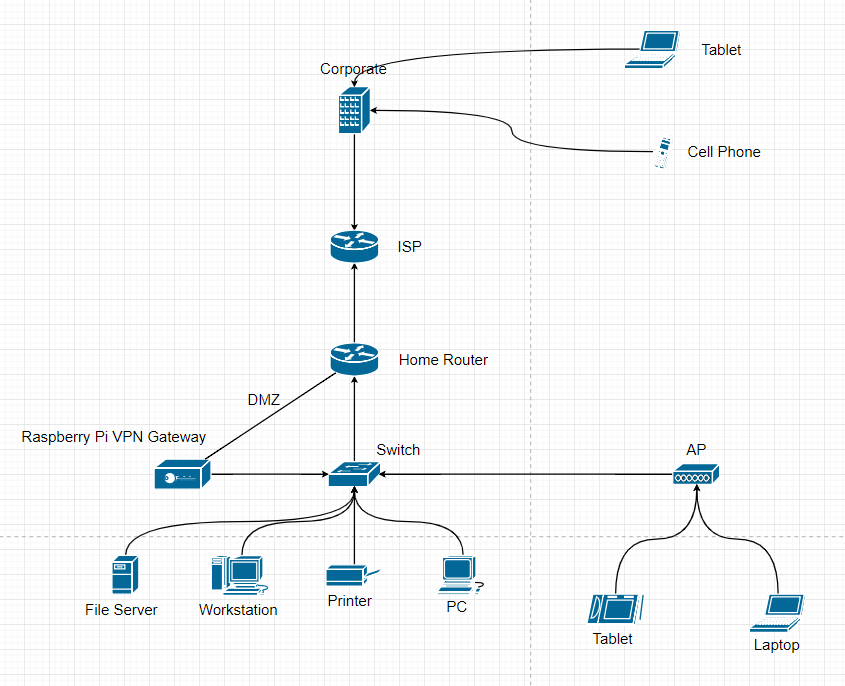
\includegraphics[scale=0.6]{topology.png}\\[1cm]
\end{center}

\subsection{Option 2: Multipurpose Gateway}

The raspberry pi will have the following roles on the network:

\begin{enumerate}
\item VPN Gateway
\item DNS Advertisement Filtering Server
\item RADIUS Server
\item Router
\item DHCP Server
\end{enumerate}

\section{Materials Needed}

The follow is a list of all the devices, component and software that are expected to be used in this project. Italic items are only applicable for option 2, when the AP and Gateway are integrated into the Raspberry Pi.

\subsection{Hardware}

Note that some of these devices are enterprise level devices. They are used throughly because \textit{Jiuxiang Lin}, a group member, is already in possession of these devices.\\

\begin{tabular}{| c | c |}
\hline
\textbf{Name} & \textbf{Quantity} \\\hline
Raspberry Pi 3 B+ & 1 \\\hline
Cisco C819G-4G-V-K9 & 1 \\\hline
Cisco WS-C3750V2-48TS-S Catalyst & 1 \\\hline
Laptop / Smart phone (as terminal devices) & As many as needed \\\hline
Ethernet cables & As many as needed \\\hline
Other minor accessories & Unknown \\\hline
\end{tabular}

\subsection{Software}

There are a number of software that we need to use for this project. To follow the thesis of this project, we try as much as we can to make use of free and open-source software.

Most of these software are expected to be pre-compiled by the Linux distribution package maintainers. Therefore it would be easy for beginners to install these packages on themselves.

\begin{enumerate}
\item ocserv
\item pi-hole
\item freeradius
\item anyradius (to be compiled)
\item \textit{hostapd}
\item \textit{isc-dhcp-server}
\end{enumerate}

\end{document}